\documentclass[/Users/ikedahajime/GitHub/reserch/master_report/thesis]{subfiles}

% このファイル内だけのコマンド
\begin{document}
\chapter{序論}

\section{研究背景}
自らの力で進むものは世の中に多く存在する。魚や鳥、人などをはじめとした生物はその典型的な例である。
%図を挿入;
\begin{figure}[htbp]
    \centering
    \begin{tabular}{c}
        \begin{minipage}{0.4\hsize}
            \text{(a)}
            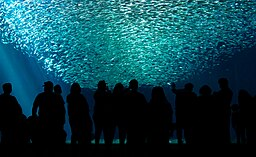
\includegraphics[width=\textwidth]{img/intro/256px-School_of_sardines_at_the_Monterey_Bay_Aquarium_(12056).jpg}
        \end{minipage}
        \begin{minipage}{0.4\hsize}
            \text{(b)}
            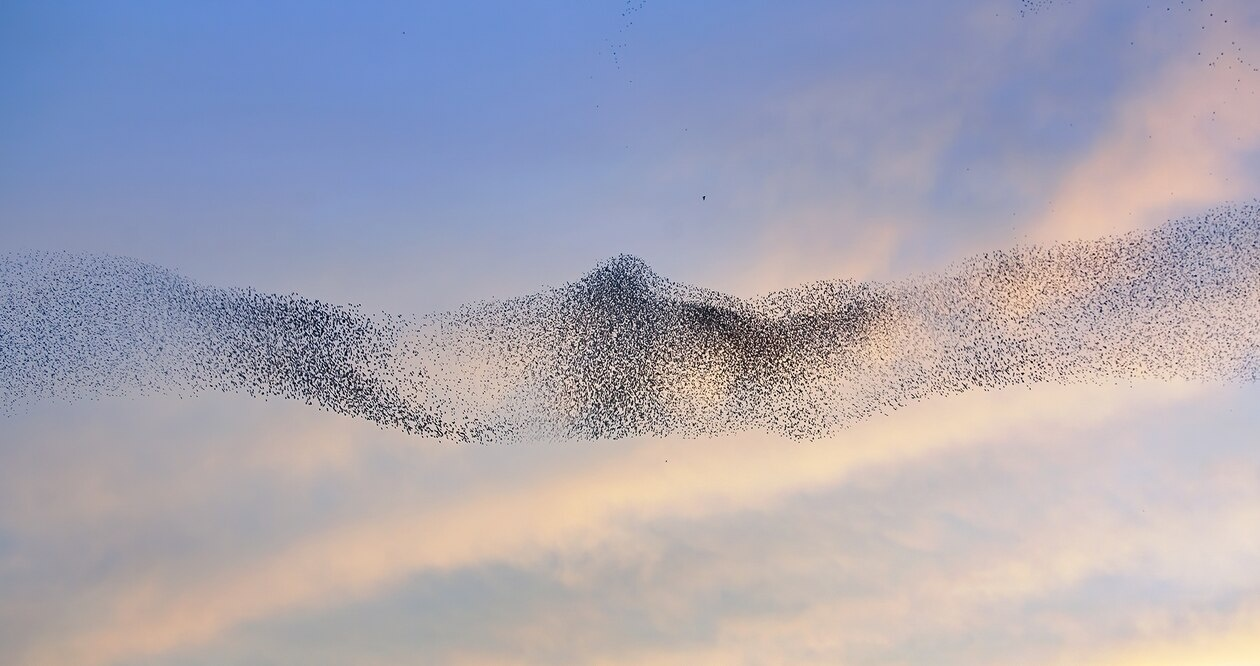
\includegraphics[width=\textwidth]{img/intro/mukudori.png}
        \end{minipage}\\
        \begin{minipage}{0.4\hsize}
            \text{(c)}
            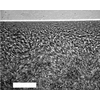
\includegraphics[width=\textwidth]{img/intro/thumbnail.png}
        \end{minipage}
    \end{tabular}
    \caption[Four sample images]
    {
        hoge
    }
    \label{fig:example_actmat}
\end{figure}
これらの生物は、単独では一見無秩序な運動を行う。しかし多くの個体が集まって集団になると、イワシのトルネード、
椋鳥の群れなどのように、群れ全体が秩序だった集団運動を行う。この集団運動は特定の個体がリーダーとなって
指示を出すことで起こっているのではなく、各個体同士の相互作用の結果として発生している。
このような自らの力で進むものやその集団のことを総称してアクティブマターと呼ぶ。アクティブマターは
環境からエネルギーを取り出し、それ自身が前を進みエネルギーを生成する。このような特徴から、非平衡な物質であるため、非平衡統計力学の
観点から近年注目を集めている。\\%TODO繋ぎ;b

アクティブマターの特徴の1つとして、自発的に渦を産むことがあげられる。
この現象は個々の構成要素が自己駆動することによって起こる現象であり、
このような系では速度相関が発達する。相関長はある特徴的な長さを持っており、
この長さは渦の大きさに関係していることがわかっている。
この現象は様々なアクティブマター系において観測されている。
例えば枯草菌\cite{wensinkMesoscaleTurbulenceLiving2012}や羊の精子\cite{creppyTurbulenceSwarmingSperm2015}
など多くの系で見ることができ、理論においてもToner-Tu-SwiftHohenberg (TTSH) 方程式など\cite{wensinkMesoscaleTurbulenceLiving2012}様々な系で見られる。%:toner-toとか
% 円領域に行った方が自然?円形領域に閉じ込めるとまわる〜
\begin{figure}[htbp]
    \centering
    \begin{tabular}{c}
        \begin{minipage}{0.4\hsize}
            \text{(a)}
            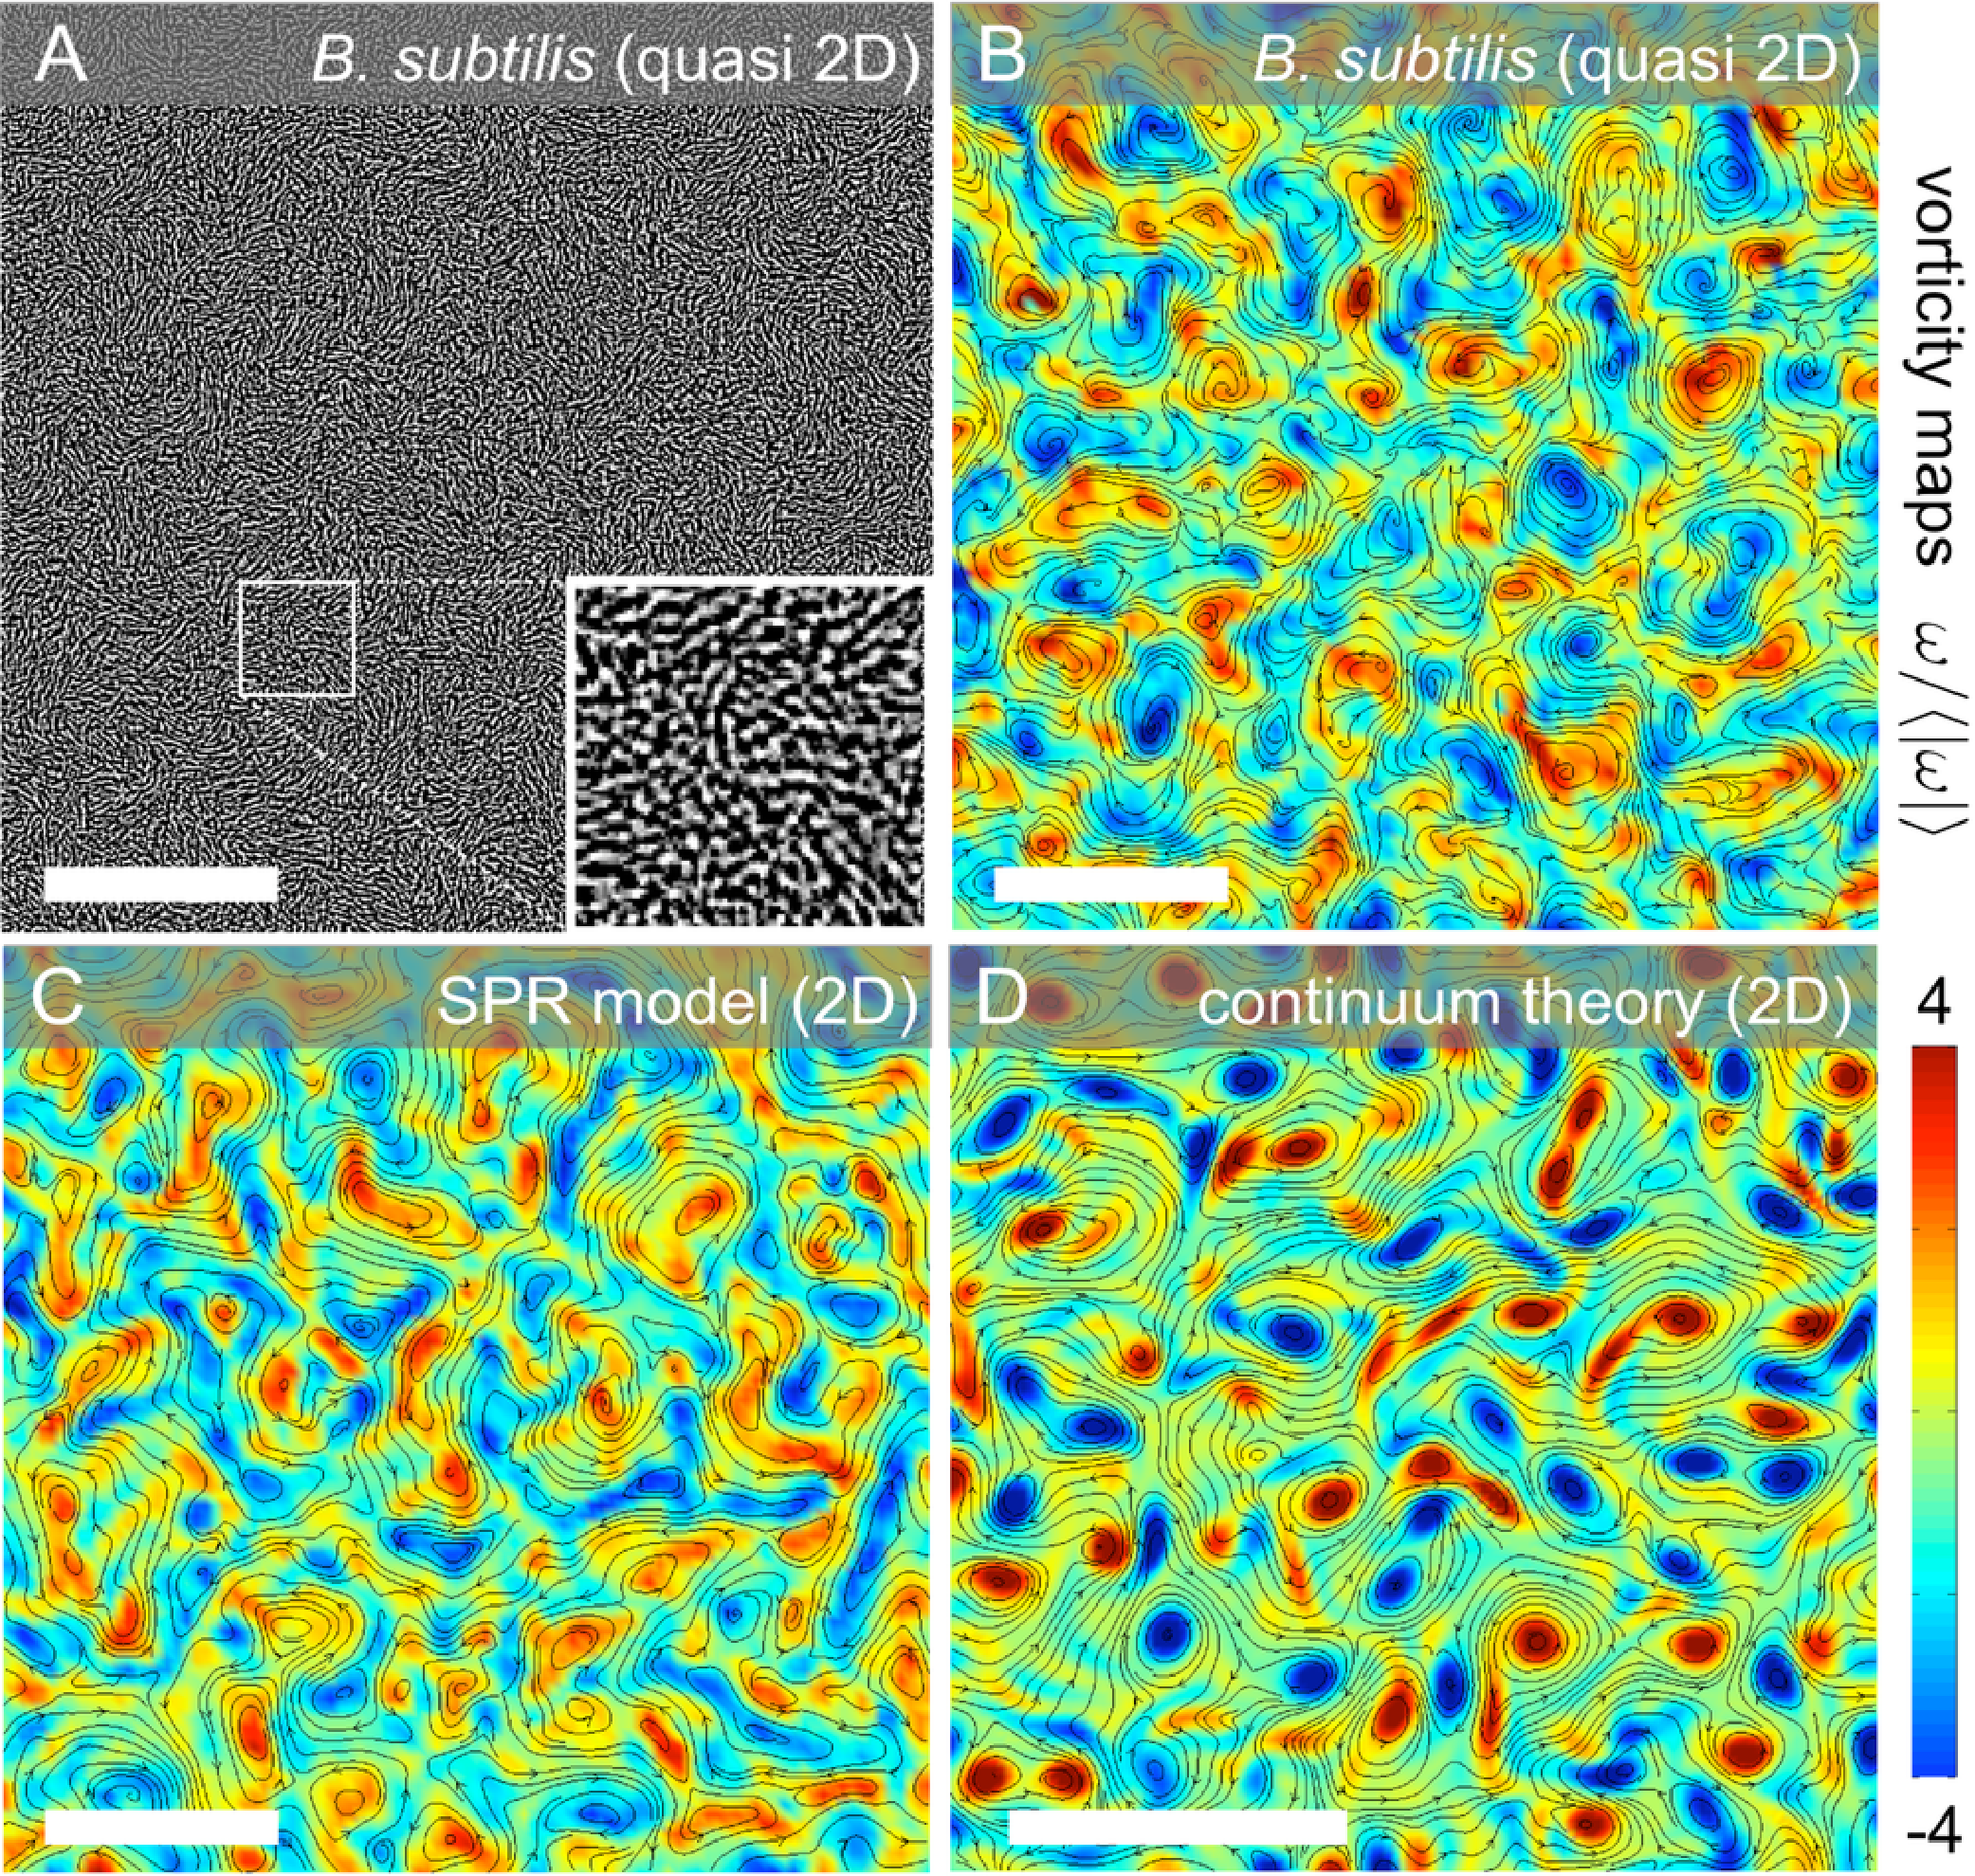
\includegraphics[width=\textwidth]{img/intro/Flow_B.subtiles.pdf}
        \end{minipage}
    \end{tabular}
    \caption[Four sample images]
    {
        hoge
    }
    \label{fig:intro_flow}
\end{figure}
\\
これらアクティブマターについての理論研究はその多くが境界のないバルク系であるが、
閉じ込め系に対する研究も行われている。閉じ込め系においてはその境界の形状などによって
様々な現象が見られている。例えば粒子の凝集\cite{dasAggregateMorphologyActive2020}、整流効果\cite{ghoshSelfPropelledJanusParticles2013}
捕集効果\cite{kaiserHowCaptureActive2012}、エッジ流\cite{soniOddFreeSurface2019}など、様々な現象が見られている。
そのような現象の1つとして、アクティブマターを円形領域の中に入れると、その
円の半径によって、円の中のアクティブマターに複数の渦ができたり全体で1つの渦になったりする。
この現象によって円の中の流れが1つになるときは、円の半径と系が持つ相関長が等しくなるところ
付近であることが知られている。
これは、この障害物とアクティブマターとの相互作用によって相関長%園内流れのず
を取り出すことができると言える。この現象は実験、理論ともに研究が進んでいるが、
理論系における研究は整列相互作用を持つモデルが主に使われている。整列相互作用のないモデルにおいては、
バルク系における速度相関の発達については見られているものの、閉じ込め系に関する研究は少ない。\\
 本研究では相関長と閉じ込めによる効果の関係を明らかにするため、
Active Brownian Particles モデル及び Chiral Active Brownian Particlesモデル
を円形領域に閉じ込めてシミュレーションを行い、円の中に生じる
流れや渦について解析を行なった。これらのモデルはシンプルなモデルであり、整列相互作用のような
複雑な相互作用が明示的に入っておらず、自己駆動性による性質を明らかにするために優れたモデルである。\\
ABP モデルの系においては、バルク系における速度相関の発達については見られており、
閉じ込め系における相関長との関係も議論されている\cite{capriniCollectiveEffectsConfined2021}。しかしこの論文では粒子をリング状の
壁に閉じ込めた一次元系であり、実験の系と比べると極端な状態であると言える。
そこで本研究では、ABPを円形領域に閉じ込めることでアクティブさ (ペクレ数) を変化させ、
系の流れについて調べた。\\
さらに、相関長と閉じ込めによる効果の関係をより明らかにするため、CABP を用いた。
CABPにおいてもバルク系における速度相関の発達については見られている。
また、このモデルをでは粒子を1つの塊にしてその塊の挙動を見る研究は行われている\cite{capriniSelfrevertingVorticesChiral2024}が、
その相関長との関係については議論されていない。
そこで、この系を円形領域に閉じ込め、粒子の回転半径 $R_\Omega$ を変化させて同様に流れや渦について調べた。


% アクティブマターとは、自らの力で進むものや、その集団のことを指す。典型的な例として、魚や鳥などの生物があげられる。
% これらの粒子は粒子自身が運動や力学的なエネルギーを産むため、平衡系の物質では観測されない、非平衡な
% 性質をもつ。\\%TODO

% アクティブマターは、外部からエネルギーを取り込み、そのエネルギーを運動や力学的な仕事に
% 変換する要素が集団を形成する系である。
% これらの要素は、個々に自己駆動性を持つ点で、受動的な粒子から成る従来の物質とは本質的に異なる。
% このエネルギー駆動の性質により、アクティブマターは平衡状態にある物質では観測されない多様な動的現象を示す。
% たとえば、鳥の群れや魚の群泳といった集団運動、細菌コロニーに見られるパターン形成、細胞骨格が示す非平衡動態などが挙げられる。
% また、近年では合成アクティブマターとして、自己駆動コロイド粒子や能動ゲルが開発され、工学的応用への可能性も広がりを見せている。
% \\
% アクティブマターの研究は、非平衡統計力学の基礎理論の構築に寄与するだけでなく、
% 生命現象の理解や次世代材料の設計にも応用可能性を持つ。
% 一方で、これらの系の動的挙動は多くの要因に依存し、特に外部環境が重要な役割を果たす。
% その中でも障害物(obstacles)は、アクティブマターの動態に多様で興味深い影響を与える要素として注目されている。
% 障害物は、アクティブ粒子の運動を妨げるだけでなく、エネルギー散逸の場として機能し、
% 粒子間の相互作用を間接的に変化させる効果を持つ。
% その結果、障害物の配置や形状に応じて、集団運動やパターン形成が大きく変化することが知られている。\\
% これまでの研究では、障害物が存在する環境におけるアクティブマターの挙動に関する多くの知見が得られている。
% たとえば、ランダムな障害物配置がアクティブ粒子の自己駆動性を低下させる「有効粘性」の増加や、
% 規則的な障害物配置が粒子の集団運動を誘起する現象が報告されている。
% また、障害物が作る狭い通路を通じた粒子の流れや、障害物周辺での粒子の蓄積など、
% 局所的な動的挙動にも興味深い特徴が見られる。しかし、障害物とアクティブ粒子の
% 相互作用に関する理論的理解や、障害物が誘発する特異な動態の統一的な記述には未解決の課題が多い。
% \\
% 本論文では、障害物を含む環境におけるアクティブマターの挙動を理論的および数値的に解析する。
% 特に、障害物の配置や形状が粒子の集団運動や動的パターン形成に及ぼす影響に焦点を当てる。
% また、障害物がアクティブマターのエネルギー消費や有効物性に与える影響についても考察する。
% 本研究は、障害物が存在する非平衡系における新たな動的現象を解明し、アクティブマター研究の発展に寄与することを目指す。


% \section{本研究の目的と方法}

% \section{本論文の構成}
本論文は以下の構成からなる。

第1章では本論文の位置づけおよび、本論文の構成について述べる.
% 第2章では本研究に関連する先行研究について説明を行う.
第2章では数値計算手法および、その設定について説明を行う.
第3,4章では本研究で得た主要な結果について述べる。
第5章では本研究の結論と今後の展望に関して述べる.
% 付録Aでは本研究の数値計算に関する予備研究について述べた.
% 付録Bでは解析手法について詳細な説明を行う。

\end{document}
